\documentclass{../../slides-style}

\slidetitleext{Лекция 7/Практика 5: Порождающие шаблоны}{18.04.2023}{Шаблоны}

\begin{document}

    \begin{frame}[plain]
        \titlepage
    \end{frame}

    \section{Паттерн ``Фабричный метод''}

    \begin{frame}
        \frametitle{``Фабричный метод'' мотивация}
        \framesubtitle{Игра-стратегия}
        \begin{columns}
            \begin{column}{0.5\textwidth}
                \begin{itemize}
                    \item Воины
                    \begin{itemize}
                        \item Мечники
                        \item Конница
                        \item Лучники
                    \end{itemize}
                    \item Хотим сделать здания, генерирующие юнитов
                \end{itemize}
            \end{column}
            \begin{column}{0.5\textwidth}
                \begin{center}
                    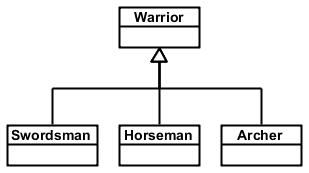
\includegraphics[width=0.8\textwidth]{warriors.png}
                \end{center}
            \end{column}
        \end{columns}
    \end{frame}

    \begin{frame}
        \frametitle{Фабричный метод}
        \begin{columns}
            \begin{column}{0.5\textwidth}
                \begin{itemize}
                    \item Базовый класс знает про остальные
                    \item switch в createWarrior()
                \end{itemize}
            \end{column}
            \begin{column}{0.5\textwidth}
                \begin{center}
                    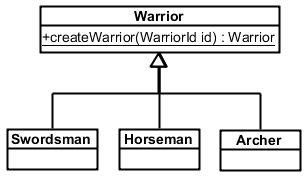
\includegraphics[width=0.8\textwidth]{warriorFactoryMethod.png}
                \end{center}
            \end{column}
        \end{columns}
    \end{frame}

    \begin{frame}
        \frametitle{Паттерн ``Factory Method''}
        \framesubtitle{Factory Method}
        \begin{center}
            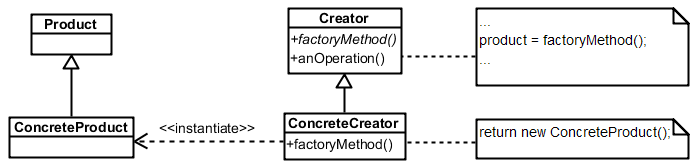
\includegraphics[width=0.8\textwidth]{factoryMethod.png}
        \end{center}
        \begin{itemize}
            \item Применимость:
            \begin{itemize}
                \item классу заранее неизвестно, объекты каких классов ему нужно создавать
                \item объекты, которые создаёт класс, специфицируются подклассами
                \item класс делегирует свои обязанности одному из нескольких вспомогательных подклассов
            \end{itemize}
        \end{itemize}
    \end{frame}

    \begin{frame}
        \frametitle{Пример, текстовый редактор}
        \begin{center}
            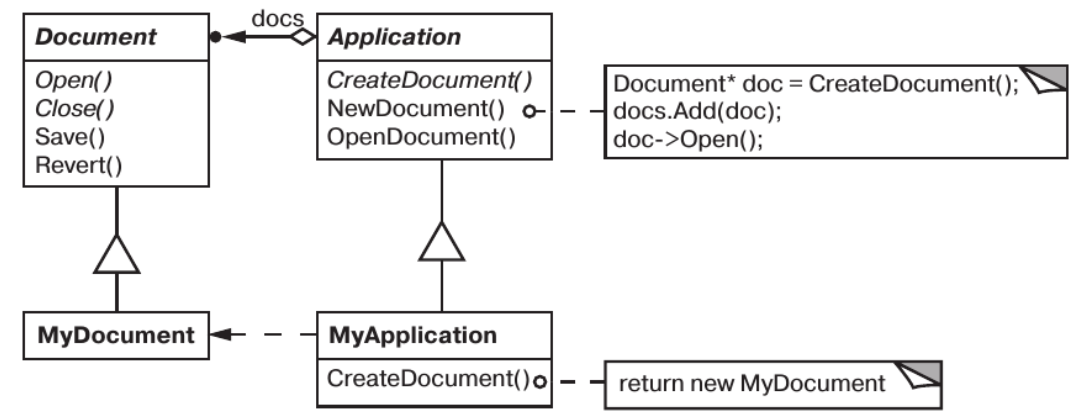
\includegraphics[width=0.9\textwidth]{factoryMethodForTextEditor.png}
        \end{center}
    \end{frame}

    \begin{frame}
        \frametitle{``Фабричный метод'', детали реализации}
        \begin{center}
            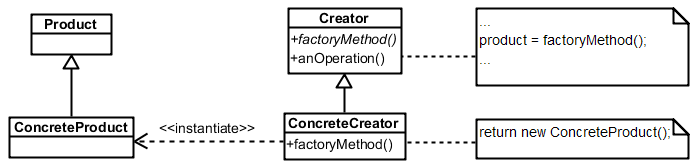
\includegraphics[width=0.6\textwidth]{factoryMethod.png}
        \end{center}
        \begin{itemize}
            \item Абстрактный Creator или реализация по умолчанию
            \begin{itemize}
                \item Второй вариант может быть полезен для расширяемости
            \end{itemize}
            \item Параметризованные фабричные методы
            \item Если язык поддерживает инстанциацию по прототипу (JavaScript, Smalltalk), можно хранить порождаемый объект
            \item Creator не может вызывать фабричный метод в конструкторе
            \item Можно сделать шаблонный Creator
        \end{itemize}
    \end{frame}

    \section{Паттерн ``Абстрактная фабрика''}

    \begin{frame}
        \frametitle{``Абстрактная фабрика'', мотивация}
        \begin{itemize}
            \item Хотим поддержать разные стили UI
            \begin{itemize}
                \item Гибкая поддержка в архитектуре
                \item Удобное добавление новых стилей
            \end{itemize}
        \end{itemize}
        \begin{center}
            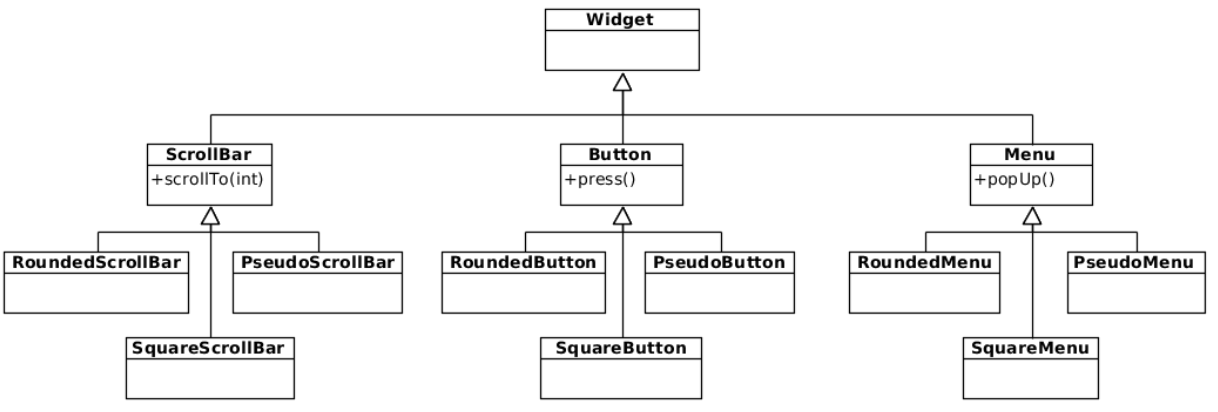
\includegraphics[width=0.95\textwidth]{widgets.png}
        \end{center}
    \end{frame}

    \begin{frame}
        \frametitle{Создание виджетов}
        \mintinline{c++}|ScrollBar* bar = new RoundedScrollBar;|
        
        \vspace{2mm}
        
        vs
        
        \vspace{2mm}
        
        \mintinline{c++}|ScrollBar* bar = guiFactory->createScrollBar();|
    \end{frame}

    \begin{frame}
        \frametitle{Фабрика виджетов}
        \begin{center}
            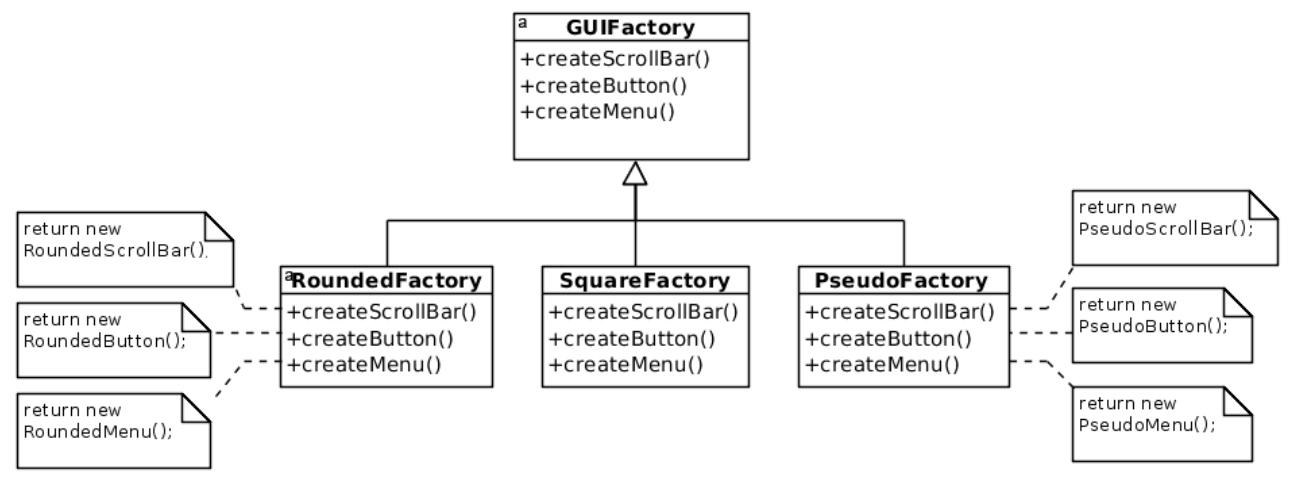
\includegraphics[width=0.95\textwidth]{widgetFactory.png}
        \end{center}
    \end{frame}

    \begin{frame}
        \frametitle{Паттерн ``Абстрактная фабрика''}
        \framesubtitle{Abstract Factory}
        \begin{columns}
            \begin{column}{0.4\textwidth}
                \begin{itemize}
                    \item Изолирует конкретные классы
                    \item Упрощает замену семейств продуктов
                    \item Гарантирует сочетаемость продуктов
                    \item Поддержать новый вид продуктов непросто
                \end{itemize}
            \end{column}
            \begin{column}{0.6\textwidth}
                \begin{center}
                    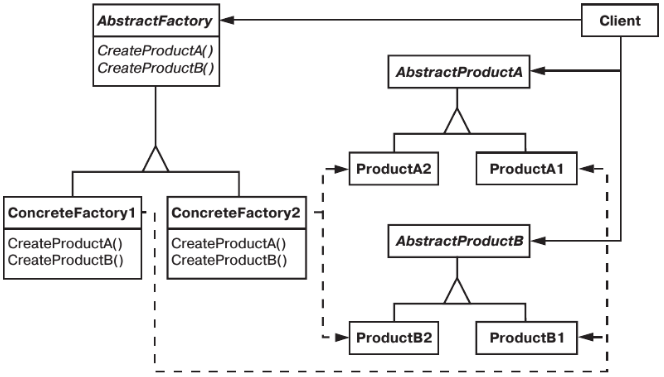
\includegraphics[width=0.95\textwidth]{abstractFactory.png}
                \end{center}
            \end{column}
        \end{columns}
    \end{frame}

    \begin{frame}
        \frametitle{``Абстрактная фабрика'', применимость}
        \begin{itemize}
            \item Система не должна зависеть от того, как создаются, компонуются и представляются входящие в неё объекты
            \item Система должна конфигурироваться одним из семейств составляющих её объектов
            \item Взаимосвязанные объекты должны использоваться вместе
            \item Хотите предоставить библиотеку объектов, раскрывая только их интерфейсы, но не реализацию
        \end{itemize}
    \end{frame}

    \begin{frame}
        \frametitle{``Абстрактная фабрика'', детали реализации}
        \begin{columns}
            \begin{column}{0.5\textwidth}
                \begin{itemize}
                    \item Хорошо комбинируются с паттерном ``Одиночка''
                    \item Если семейств продуктов много, то фабрика может инициализироваться \textit{прототипами}, тогда не надо создавать сотню подклассов
                \end{itemize}
            \end{column}
            \begin{column}{0.5\textwidth}
                \begin{center}
                    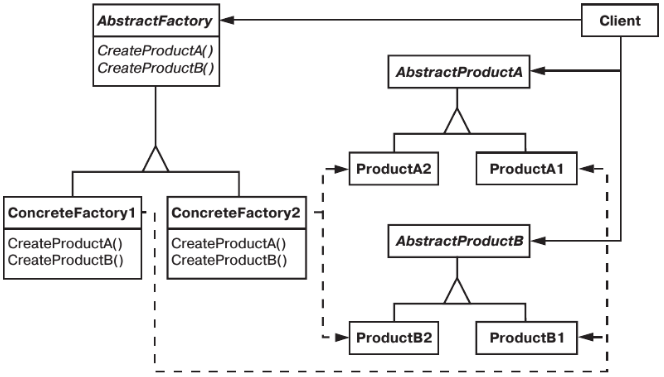
\includegraphics[width=\textwidth]{abstractFactory.png}
                \end{center}
            \end{column}
        \end{columns}
        \begin{itemize}
            \item Прототип на самом деле может быть классом (например, Class в Java)
            \item Если виды объектов часто меняются, может помочь параметризация метода создания
            \begin{itemize}
                \item Может пострадать типобезопасность
            \end{itemize}
        \end{itemize}
    \end{frame}

    \section{Паттерн ``Прототип''}

    \begin{frame}
        \frametitle{``Прототип'', мотивация}
        \begin{center}
            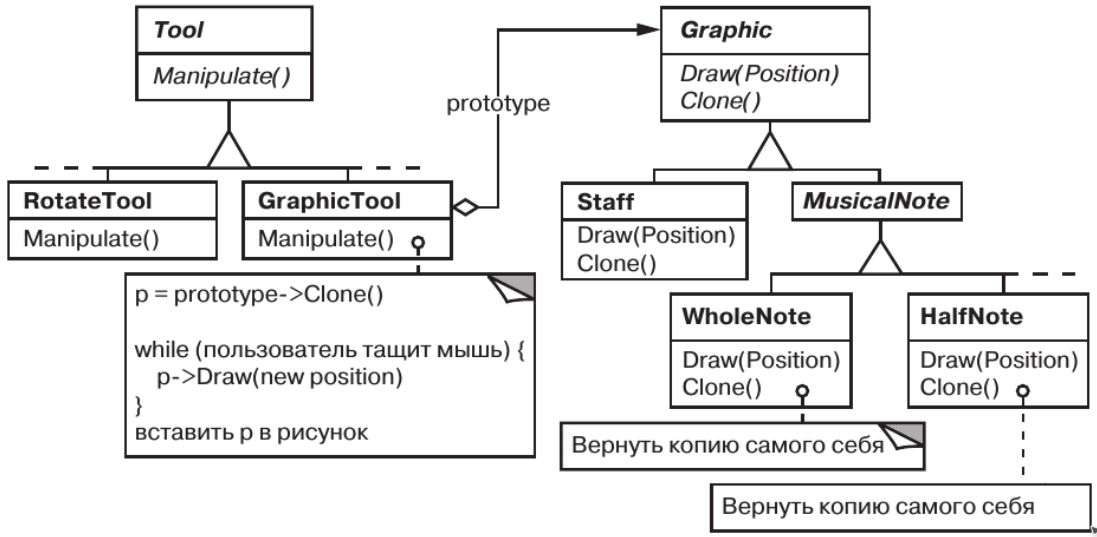
\includegraphics[width=0.9\textwidth]{musicalEditor.png}
        \end{center}
    \end{frame}

    \begin{frame}
        \frametitle{Паттерн ``Прототип''}
        \framesubtitle{Prototype}
        \begin{center}
            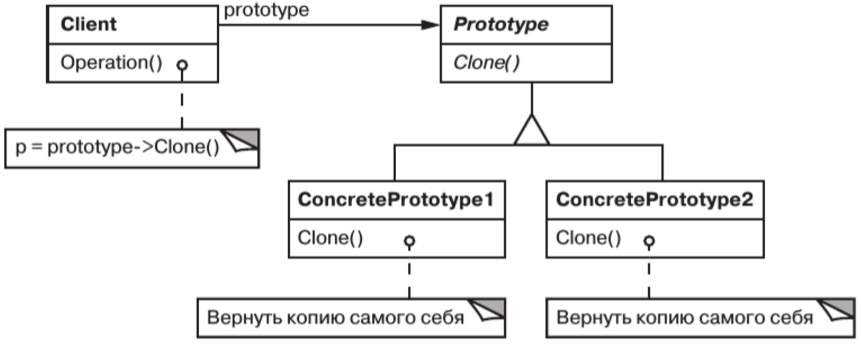
\includegraphics[width=0.85\textwidth]{prototype.png}
        \end{center}
    \end{frame}
    
    \begin{frame}
        \frametitle{``Прототип'', детали реализации}
        \begin{itemize}
            \item Реестр прототипов, обычно ассоциативное хранилище
            \item Операция Clone
            \begin{itemize}
                \item Глубокое и мелкое копирование
                \item В случае, если могут быть круговые ссылки
                \item Сериализовать/десериализовать объект (но помнить про идентичность)
            \end{itemize}
            \item Инициализация клона
            \begin{itemize}
                \item Передавать параметры в Clone --- плохая идея
            \end{itemize}
        \end{itemize}
    \end{frame}

    \section{Паттерн ``Строитель''}

    \begin{frame}
        \frametitle{``Строитель'', мотивация}
        \framesubtitle{Конвертер текста}
        \begin{center}
            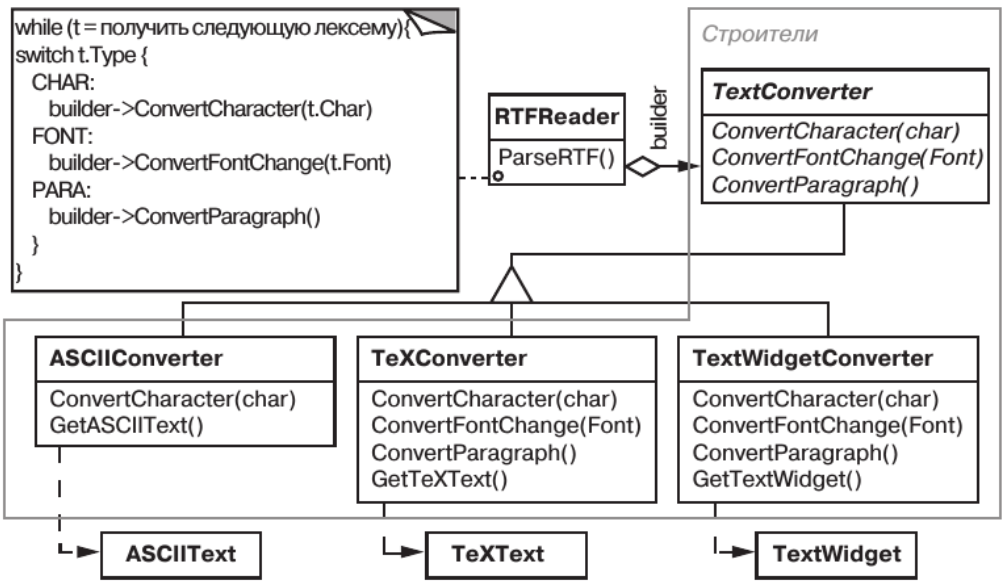
\includegraphics[width=0.8\textwidth]{textConverter.png}
        \end{center}
    \end{frame}

    \begin{frame}
        \frametitle{Паттерн ``Строитель''}
        \framesubtitle{Builder}
        \begin{center}
            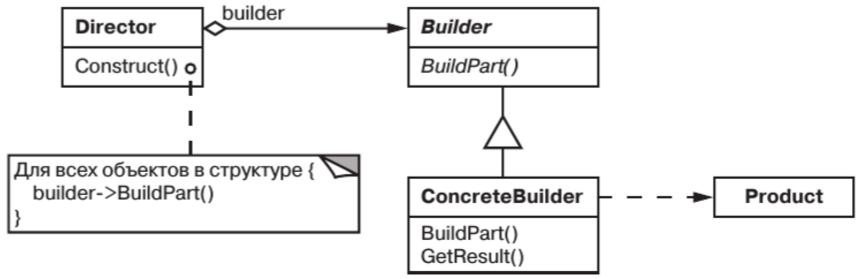
\includegraphics[width=0.85\textwidth]{builder.png}
        \end{center}
    \end{frame}
    
    \begin{frame}
        \frametitle{``Строитель'' (Builder), детали реализации}
        \begin{center}
            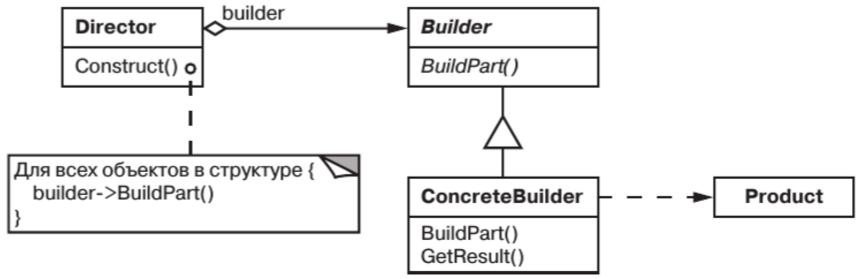
\includegraphics[width=0.7\textwidth]{builder.png}
        \end{center}
        \begin{itemize}
            \item Абстрактные и конкретные строители
            \begin{itemize}
                \item Достаточно общий интерфейс
            \end{itemize}
            \item Общий интерфейс для продуктов не требуется
            \begin{itemize}
                \item Клиент конфигурирует распорядителя конкретным строителем, он же и забирает результат
            \end{itemize}
            \item Пустые методы по умолчанию
        \end{itemize}
    \end{frame}

    \begin{frame}[fragile]
        \frametitle{``Строитель'', примеры}
        \begin{itemize}
            \item StringBuilder
            \item Guava, подсистема работы с графами
            \begin{minted}{java}
MutableNetwork<Webpage, Link> webSnapshot = 
        NetworkBuilder.directed()
    .allowsParallelEdges(true)
    .nodeOrder(ElementOrder.natural())
    .expectedNodeCount(100000)
    .expectedEdgeCount(1000000)
    .build();
            \end{minted}
        \end{itemize}
    \end{frame}

    \section{Задание}

    \begin{frame}
        \frametitle{Задание на остаток пары}
        Уточнить модель компьютерной игры Roguelike:

        \begin{enumerate}
            \item Используя шаблон ``Строитель'' для инициализации карты
            \item Используя шаблон ``Абстрактная фабрика'' для создания мобов и предметов на карте
            \item Используя шаблон ``Прототип'' для поддержки клонирования персонажей и предметов
        \end{enumerate}

        Выложить модифицированные диаграммы классов в Teams
    \end{frame}

\end{document}
